\documentclass[11pt]{article}
\usepackage{../../Utility/Template}
\usepackage{hyperref}
\usepackage{fancyhdr}
\usepackage[shortlabels]{enumitem}
\usepackage[raggedright]{titlesec}

\setcounter{secnumdepth}{4}
\setcounter{tocdepth}{4}
\definecolor{apricot}{rgb}{0.94, 0.87, 0.8}

\begin{document}
\newcommand{\Titolo}{\Glossario}

\newcommand{\Redattori}{\SP{} \newline	\ZM{} \newline \RA{} \newline \SH{}}

\newcommand{\Verificatori}{\BM{} \newline \PA{}}

\newcommand{\Approvatore}{\SG{}}

\newcommand{\Distribuzione}{\Proponente{} \newline \VT{} \newline \CR{} \newline Gruppo \Gruppo{}}

\newcommand{\Uso}{Esterno}

\newcommand{\DescrizioneDoc}{Il glossario serve per dare una definizione e chiarire il significato di alcuni termini presenti nella documentazione fornita.}

\newcommand{\pathimg}{../../Utility/images/logo2.png}

\newcommand{\Versionedoc}{1.0.0}
% info generali 

\newcommand{\NomeProgetto}{\textit{HD Viz}}

% fornitore
\newcommand{\Gruppo}{\textit{CodeBusters}}
\newcommand{\Mail}{codebusterswe@gmail.com}

% committenti
\newcommand{\Committente}{\VT \newline \CR}
\newcommand{\VT}{Prof. Vardanega Tullio}
\newcommand{\CR}{Prof. Cardin Riccardo}

% proponenti
\newcommand{\Proponente}{\textit{Zucchetti}}

% codebusters
\newcommand{\SG}{Sassaro Giacomo}
\newcommand{\BM}{Baldisseri Michele}
\newcommand{\ZM}{Zenere Marco}
\newcommand{\PA}{Pirolo Alessandro}
\newcommand{\SP}{Scialpi Paolo}
\newcommand{\SH}{Safdari Hossain}
\newcommand{\RA}{Rago Alessandro}

% ruoli
\newcommand{\Responsabile}{Responsabile di Progetto}
\newcommand{\Amministratore}{Amministratore di Progetto}

% documenti

\newcommand{\SdF}{\textit{Studio di Fattibilità}}
\newcommand{\SdFv}[1]{\textit{Studio di Fattibilità {#1}}}
\newcommand{\PdQ}{\textit{Piano di Qualifica}}
\newcommand{\PdQv}[1]{\textit{Piano di Qualifica {#1}}}
\newcommand{\PdP}{\textit{Piano di Progetto}}
\newcommand{\PdPv}[1]{\textit{Piano di Progetto {#1}}}
\newcommand{\NdP}{\textit{Norme di Progetto}}
\newcommand{\NdPv}[1]{\textit{Norme di Progetto {#1}}}
\newcommand{\AdR}{\textit{Analisi dei Requisiti}}
\newcommand{\AdRv}[1]{\textit{Analisi dei Requisiti {#1}}}
\newcommand{\Glossario}{\textit{Glossario}}
\newcommand{\Glossariov}[1]{\textit{Glossario {#1}}}
\newcommand{\MM}{\textit{Manuale Manutentore}}
\newcommand{\MMv}[1]{\textit{Manuale Manutentore {#1}}}
\newcommand{\MU}{\textit{Manuale Utente}}
\newcommand{\MUv}[1]{\textit{Manuale Utente {#1}}}

% comandi generali
\newcommand{\glo}[1]{#1\ap{G}}
%\newcommand{\glo}[1]{\textsc{#1\textsuperscript{\textit{G}}}}

\setlength{\parindent}{-0.1em}
\frontespizio
\fancydoc
\newpage	
\section*{Registro delle modifiche}
{
\rowcolors{2}{colorePanna}{coloreGrigietto}
\renewcommand{\arraystretch}{1.5}
\centering
\begin{longtable}{c C{2.6cm} C{3cm} C{3cm} C{5cm}}
\rowcolor{coloreRosso}
\textcolor{white}{\textbf{Versione}}&
\textcolor{white}{\textbf{Data}}&
\textcolor{white}{\textbf{Nominativo}}&
\textcolor{white}{\textbf{Ruolo}}&
\textcolor{white}{\textbf{Descrizione}}\\	
\endhead

1.0.0 & 08/01/2021 & \SG{} & Responsabile & Approvazione del documento \\

0.3.0 & 04/01/2021 & \SH{} & Verificatore & Revisione complessiva del documento \\

0.2.6 & 22/12/2020 & \BM{} & Responsabile & Stesura \S A e \S B \\

0.2.5 & 21/12/2020 & \BM{} & Responsabile & Stesura \S 6\\

0.2.4 & 21/12/2020 & \SG{} & Responsabile & Aggiunti grafici \\

0.2.3 & 21/12/2020 & \BM{} & Responsabile & Stesura \S 5.3 e \S 5.4\\

0.2.2 & 20/12/2020 & \SG{} & Responsabile & Fine stesura \S 5.2 e stesura \S 5.5 \\

0.2.1 & 20/12/2020 & \BM{} & Responsabile & Stesura \S 5.3 e \S 5.4\\

0.2.0 & 19/12/2020 & \ZM{} & Verificatore & Revisione complessiva del documento \\

0.1.6 & 19/12/2020 & \SG{} & Responsabile & Inizio stesura \S 5 \\

0.1.5 & 18/12/2020 & \PA{} & Amministratore & Fine stesura \S 4.3\\

0.1.4 & 18/12/2020 & \SG{} & Responsabile & Stesura \S 4.4 \\

0.1.3 & 17/12/2020 & \BM{} & Responsabile & Stesura \S 4.2 e iniziata \S 4.3 \\

0.1.2 & 17/12/2020 & \SG{} & Responsabile & Stesura \S 4.1 \\

0.1.1 & 17/12/2020 & \SG{},\newline \BM{} & Responsabili & Stesura \S 3.2 \\

0.1.0 & 17/12/2020 & \ZM{} & Verificatore & Revisione complessiva del documento \\

0.0.5 & 16/12/2020 & \BM{} & Responsabile & Stesura \S 2.2 e \S 2.3 \\
		
0.0.4 & 15/12/2020 & \PA{} & Amministratore & Inizio stesura \S 2 \\

0.0.3 & 15/12/2020 & \SG{} & Responsabile & Stesura \S 3.1 \\

0.0.2 & 14/12/2020 & \PA{} & Amministratore & Aggiunta \S 1 \\

0.0.1 & 14/12/2020 & \SG{} & Responsabile & Creata struttura del documento Latex \\
		
\end{longtable}
}

\newpage
\tableofcontents
\newpage
\listoftables
\newpage
\listoffigures
\newpage
\section{Introduzione}
\subsection{Scopo del documento}
Questo documento ha lo scopo di fornire tutte le informazioni relative al sistema di controllo di qualità per i processi ed i prodotti, basandosi su assunti misurabili ma adattati alle esigenze del proprio progetto.
Esso deve implementare degli standard che permettano il miglioramento continuo, tracciando periodicamente tramite misurazioni i risultati ottenuti sfruttandoli per definire azioni migliorative. All'interno del \textit{Piano di Qualifica} vengono anche raccolte le definizioni dei test, il loro stato e il loro tracciamento. 

\subsection{Scopo del capitolato}
Oggigiorno, anche i programmi più tradizionali gestiscono e memorizzano una grande mole di dati; di conseguenza servono software in grado di eseguire un'analisi e un'interpretazione delle informazioni.\\
Il \glo{capitolato} C4 ha come obiettivo quello di creare un'applicazione di visualizzazione di dati con numerose dimensioni in modo da renderle comprensibili all'occhio umano.  Lo scopo del prodotto sarà quello di fornire all'utente diversi tipi di visualizzazioni e di algoritmi per la riduzione dimensionale in modo che, attraverso un processo esplorativo, l'utilizzatore del prodotto possa studiare tali dati ed evidenziarne degli eventuali \glo{cluster}. 

\subsection{Glossario}
Per evitare ambiguità relative alle terminologie utilizzate, è stato compilato il \Glossariov{2.0.0}. In questo documento sono riportati tutti i termini importanti e con un significato particolare. Questi termini sono evidenziati da una 'G' ad apice.

\subsection{Riferimenti}
\subsubsection{Riferimenti normativi}
\begin{itemize}	
\item \textbf{\NdPv{v 2.0.0}};
	
\item \textbf{Capitolato d'appalto C4 - HD Viz: visualizzazione di dati multidimensionali}:\\
	\textcolor{blue}{\url{https://www.math.unipd.it/~tullio/IS-1/2020/Progetto/C4.pdf}}

\end{itemize}

\subsubsection{Riferimenti informativi}
\begin{itemize}
	\item \textbf{Software Engineering - Ian Sommerville - 10 th Edition}: \\
	Parte 4 - Software Management
	\begin{itemize}
	\item Capitolo 24 - Quality Management:
		\begin{itemize}
			\item Paragrafo 24.1 - Software Quality (da pag. 703 a 705);
			\item Paragrafo 24.3 - Reviews and inspection (da pag. 710 a 714);
			\item Paragrafo 24.5 - Software measurement (da pag. 717 a 725).
		\end{itemize}
	\end{itemize}
	
	\item \textbf{Slide T12 del corso Ingegneria del Software - Qualità di prodotto}:\\
	\textcolor{blue}{\url{https://www.math.unipd.it/~tullio/IS-1/2020/Dispense/L12.pdf}}
	\begin{itemize}
		\item Slide 8 - I 7 principi del Sistema Qualità;
		\item Slide 12,13 - Cosa significa qualità SW;
		\item Slide 17 - Il processo di valutazione.
	\end{itemize}
	
	\item \textbf{Slide T13 del corso Ingegneria del Software - Qualità di processo}:\\
	\textcolor{blue}{\url{https://www.math.unipd.it/~tullio/IS-1/2020/Dispense/L13.pdf}}
		\begin{itemize}
		\item Slide 3 - Modello concettuale di processo;
		\item Slide 11 - I 5 livelli di maturità;
		\item Slide 23 - Riepilogo: la ricerca della qualità.
	\end{itemize}
	
	\item \textbf{Slide T14 del corso Ingegneria del Software - Verifica e validazione}:\\
	\textcolor{blue}{\url{https://www.math.unipd.it/~tullio/IS-1/2020/Dispense/L14.pdf}}
	\begin{itemize}
		\item Slide 6 - Verifica e validazione nello sviluppo; 
		\item Slide 15 - Analisi dinamica: tipi di test.
	\end{itemize}
	
	\item \textbf{Indice di Gulpease}:\\
	\textcolor{blue}{\url{https://it.wikipedia.org/wiki/Indice_Gulpease}}
	
	\item \textbf{Averege Cyclomatic complexity}:\\
	\textcolor{blue}{\url{https://eslint.org/docs/rules/complexity}}
	
\end{itemize}
\newpage
\section{Descrizione Generale}
\subsection{Obiettivi del prodotto}
L'obiettivo del progetto è la realizzazione di un'applicazione che permette la visualizzazione di dati a molte dimensioni, come supporto della fase esplorativa della loro analisi, con l'utilizzo di tecnologie web.
\subsection{Funzioni del prodotto}
L'applicazione si occupa di analizzare dati a molte dimensioni e di restituire dei grafici che, grazie all'aiuto di specifici algoritmi di riduzione dimensionale, risultano essere più comprensibili e significativi. In questo modo il grafico scelto dall'utente può diventare molto utile per estrapolare informazioni che in un primo momento potevano essere nascoste o poco chiare. I \glo{dataset} possono essere reperiti dall'apposito \glo{database} oppure possono essere caricati dall'utente nel caso in cui ne possieda in formato \glo{CSV}. Per agevolare il processo esplorativo, l'utente ha la possibilità, in base al grafico scelto, di apportare alcune modifiche in modo da raffinare l'elaborazione sullo specifico set di dati in esame.\\ Per un'eventuale gestione di dati in più sessioni di lavoro, sarà possibile salvare le informazioni in un file scaricabile, che potrà essere successivamente caricato sulla piattaforma ripristinando la sessione nel punto in cui era stata interrotta.

\subsection{Database}
Visto il potenziale di questa web app per l'analisi dei dati, in reali contesti lavorativi la quantità di \glo{dataset} studiati sarà notevole, ciascuno costituito da molti campi e valori. Per questa ragione la presenza di un database, contenente tutti i dataset raggiungibili tramite \glo{query}, risulta essere essenziale e l'utilizzo di file \glo{CSV} sarà solo l'eccezione. \\
La web app dovrà essere predisposta per la comunicazione con un database, di tipo relazionale, solamente per la ricezione dei dati; la sua gestione di amministrazione e mantenimento sarà gestita separatamente e non è richiesta come vincolo.

\subsection{Caratteristiche degli utenti}
Il progetto non prevede come requisito la presenza di diverse categorie di utenza e non è necessaria una funzionalità di autenticazione: chiunque ha accesso alle complete funzionalità del prodotto. 
\subsection{Piattaforme di esecuzione}
Il progetto sarà costituito da un insieme di pagine web accessibili dai browser più diffusi, nelle loro versioni recenti, come \glo{Google Chrome}, \glo{Mozilla Firefox}, \glo{Safari} o \glo{Edge}. Non è richiesto, come requisito, una completa compatibilità con browser meno diffusi.

\newpage

\subsection{Vincoli di progettazione}

\renewcommand{\arraystretch}{1.5}
\begin{longtable}{C{4cm} | C{11.5cm}}
		\rowcolor{coloreRosso}
		\textcolor{white}{\textbf{Tipologia}} & 
		\textcolor{white}{\textbf{Descrizione}} \\
		\endfirsthead
	    \rowcolor{white}\multicolumn{2}{c}{\textit{Continua nella pagina successiva...}}\\
	    \endfoot
	    \rowcolor{white}\caption{Tabella dei requisiti di progettazione}
	    \endlastfoot

\rowcolor{coloreRossoChiaro}\multicolumn{2}{c}{\textcolor{white}{\textbf{Requisiti obbligatori}}}\\	    
	    
Implementazione del \glo{front-end} & Utilizzo di \glo{HTML}, \glo{CSS} e \glo{JavaScript}\\

Implementazione dei grafici & Utilizzo della libreria \glo{D3.js} per creare visualizzazioni almeno fino a 15 dimensioni\\

Tipi di grafici & 
1. \glo{Scatter plot Matrix} (massimo 5 dimensioni);
\newline 2. \glo{Force Field}  ;
\newline 3. \glo{Heat Map} (con ordinamento dei dati per evidenziare i \glo{cluster});
\newline 4. \glo{Proiezione Lineare Multi Asse} 
\\

Recupero dati & Il sistema deve accettare dati sia tramite \glo{query} ad un database che caricamento di file in formato \glo{CSV} \\

Implementazione del \glo{back-end} & Utilizzo di un \glo{database} \glo{SQL} o \glo{NoSQL} con server \glo{Tomcat} o \glo{Node.js} \\
	    
\rowcolor{coloreRossoChiaro}\multicolumn{2}{c}{\textcolor{white}{\textbf{Requisiti opzionali}}}\\	

Tipi di grafici & Implementazione di altri grafici adatti alla visualizzazione dei dati con più di tre dimensioni \\

Modifiche alla visualizzazione & 1. Utilizzo di funzioni di calcolo della distanza diverse dalla \glo{distanza “Euclidea”}; \newline
2. Utilizzo di funzioni di “forza” diverse da quelle previste in automatico dal grafico “Force Based” di \glo{D3.js} \\

Preparazione dei dati & 1. Utilizzo di algoritmi di pulizia dei dati poco rilevanti; \newline
2. Analisi automatiche per evidenziare situazioni di particolare interesse\\

\end{longtable}




\newpage
\section{Casi d'uso}
\subsection{Scopo}
Lo scopo di questa sezione è la descrizione in elenco di tutti i casi d'uso individuati dal gruppo, in riferimento alle funzionalità dell'applicazione.
\subsection{Attori}
Come accordato con il proponente, non essendo richiesto alcun servizio di autenticazione attraverso un login o una registrazione, è presente un solo attore che può interagire con l'applicazione web:

\begin{figure}[h]
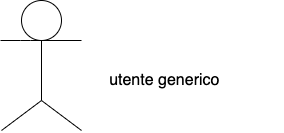
\includegraphics[width=1cm]{section/Images/Utente.png}
\centering
\caption{Gerarchia attori}
\end{figure}

\begin{description}
\item[Utente]:
Si riferisce all'utente utilizzatore che può accedere alla piattaforma.
\end{description}
Per un eventuale gestione di dati in più sessioni è quindi richiesta la funzionalità di poter salvare il proprio lavoro in un file scaricabile, che può poi essere successivamente caricato sulla piattaforma permettendo la ripresa del lavoro.
\subsection{Elenco casi d'uso}
\subsubsection{UC1 - Caricamento del dataset}
\begin{figure}[h]
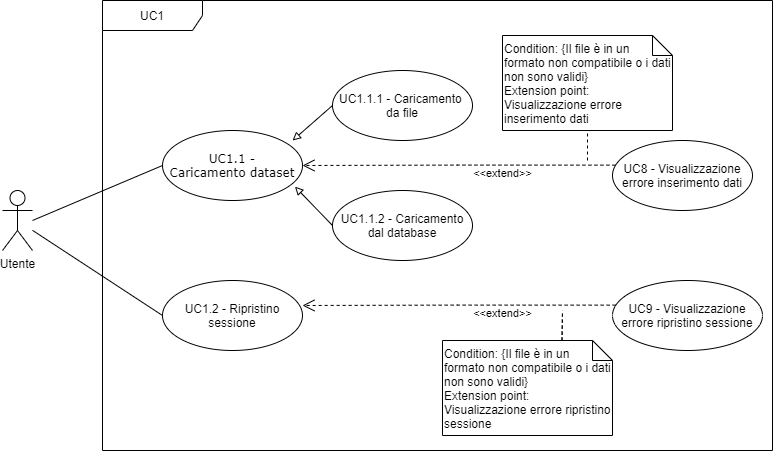
\includegraphics[width=\linewidth]{section/Images/UC1.png}
\centering
\caption{UC1 - Caricamento del dataset}
\end{figure}
\begin{itemize}
	\item \textbf{Attore primario}: Utente.
	\item \textbf{Precondizioni}: Il sistema è raggiungibile e funzionante.
	\item \textbf{Postcondizioni}: Viene visualizzato un messaggio che avvisa l'utente del corretto caricamento dei dati e della loro validità.
	\item \textbf{Scenario principale}:
		\begin{enumerate}
			\item L'utente accede al sistema;
			\item L'utente sceglie come ricavare i dati:
				\begin{enumerate}[(a)]
			\item L'utente seleziona la funzionalità "carica file" [UC1.1];
			\item L'utente seleziona un dataset tra quelli disponibili nel database [UC1.2].
				\end{enumerate}
		\end{enumerate}
	\item \textbf{Estensioni}:
	\begin{enumerate}[(a)]
		\item Nel caso in cui il file sia in un formato sbagliato o i dati non sono validi:
		\begin{enumerate}[1.]
			\item i dati non vengono caricati nel sistema;
			\item viene visualizzato un errore esplicativo [UC7].
		\end{enumerate}
	\end{enumerate}
\end{itemize}

\subsubsection{UC1.1 - Caricamento dataset da file}

\begin{itemize}
	\item \textbf{Attore primario}: Utente.
	\item \textbf{Precondizioni}: Il sistema è raggiungibile e funzionante. L'utente ha a disposizione un dataset in formato CSV.
	\item \textbf{Postcondizioni}: I dati presenti nel file vengono caricati nel sistema. Viene visualizzato un messaggio che avvisa l'utente del corretto caricamento e della validità dei dati.
	\item \textbf{Scenario principale}: L'utente sceglie di caricare un dataset personale o ricavato da altre fonti esterne.
	
\end{itemize}

\subsubsection{UC1.2 - Caricamento dataset dal database}

\begin{itemize}
	\item \textbf{Attore primario}: Utente.
	\item \textbf{Precondizioni}: Il sistema è raggiungibile e funzionante. L'utente effettua una query dal database disponibile per prelevare il dataset.
	\item \textbf{Postcondizioni}: I dati vengono caricati nel sistema. Viene visualizzato un messaggio che avvisa l'utente del corretto caricamento e della loro validità.
	\item \textbf{Scenario principale}: L'utente sceglie di caricare un dataset tra quelli presenti nel database.
	
\end{itemize}


  
\subsection{UC2 - Selezione delle dimensioni da utilizzare}
\begin{itemize}
	\item \textbf{Attore primario}: Utente;
	\item \textbf{Precondizioni}: L'utente ha caricato i dati nel sistema [UC1];
	\item \textbf{Postcondizioni}: Le dimensioni scelte vengono aggiornate nel sistema e i dati sono pronti per essere visualizzati [UC6];
	\item \textbf{Scenario principale}:
		\begin{enumerate}
			\item All'utente viene presentata una schermata con tutte le dimensioni presenti nel dataset caricato già selezionate di default;
			\item Per ogni dimensione è presente una cella da selezionare nel caso la si voglia utilizzare o meno;
			\item L'utente seleziona le dimensioni che desidera analizzare.
		\end{enumerate}
	\item \textbf{Estensioni:}
		\begin{enumerate}[(a)]
			\item Nel caso in cui l'utente non abbia selezionato nessuna dimensione:
			\begin{enumerate}[1.]
				\item Le dimensioni non vengono aggiornate nel sistema;
				\item Viene visualizzato un messaggio d'errore esplicativo [UC12].
			\end{enumerate}
		\end{enumerate}
\end{itemize}
\newpage
\subsubsection{UC3 - Scelta della \glo{visualizzazione}}
\begin{figure}[h]
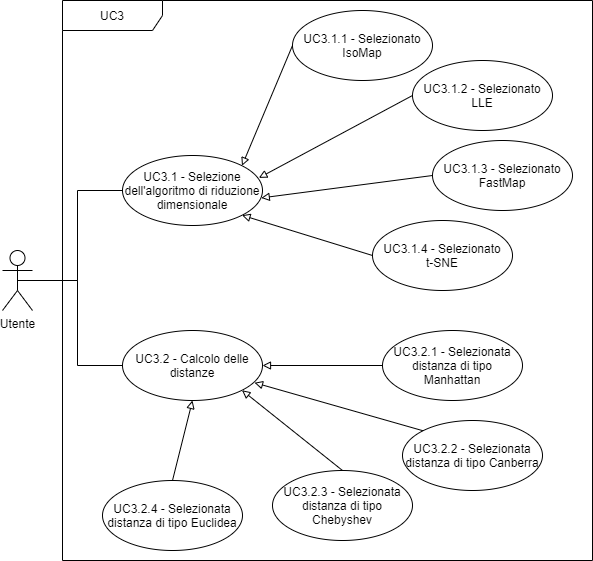
\includegraphics[width=\linewidth]{section/Images/UC3.png}
\centering
\caption{UC3 - Scelta della visualizzazione}
\end{figure}
\begin{itemize}
	\item \textbf{Attore primario}: Utente.
	\item \textbf{Precondizioni}: L'utente ha caricato dei dati nel sistema [UC1] e ha selezionato le dimensioni da utilizzare [UC2].
	\item \textbf{Postcondizioni}: Viene mostrata la visualizzazione scelta, con possibilità di personalizzazione [UC4].
	\item \textbf{Scenario principale}: L'utente seleziona una visualizzazione tra quelle disponibili.
	\item \textbf{Generalizzazioni}: L'utente seleziona una delle seguenti opzioni disponibili:
		\begin{enumerate}[(a)]
			\item \glo{\textit{Scatter Plot Matrix}} [UC3.1]
			\item \glo{\textit{Heat Map}} [UC3.2]
			\item \glo{\textit{Force Field}} [UC3.3]
			\item \glo{\textit{Proiezione Lineare Multi Asse}} [UC3.4]
		\end{enumerate}
	\item \textbf{Estensioni}:
	\begin{enumerate}[(a)]
		\item Nel caso in cui non è stato caricato alcun dato o non è stata scelta alcuna dimensione:
		\begin{enumerate}[1.]
			\item Il grafico non viene visualizzato;
			\item Viene visualizzato un errore esplicativo [UC9].
		\end{enumerate}
	\end{enumerate}
\end{itemize}
\subsubsection{UC3.1 - Scelta dell'algoritmo di riduzione dimensionale}
\begin{itemize}
	\item \textbf{Attore primario}: Utente;
	\item \textbf{Precondizioni}: L'utente ha caricato i dati e le dimensioni nel sistema [UC1];
	\item \textbf{Postcondizioni}: La scelta viene memorizzata nel sistema e viene resa disponibile una sezione per la personalizzazione dei parametri dell'algoritmo di riduzione dimensionale selezionato [UC4];
	\item \textbf{Scenario principale}: L'utente seleziona un algoritmo di riduzione dimensionale tra quelli resi disponibili dal sistema.
	\item \textbf{Generalizzazioni}: L'utente seleziona una delle seguenti opzioni:
	\begin{enumerate}[1.]
		\item \glo{\textit{Isometric Mapping (IsoMap)}} [UC3.1.1];
		\item \glo{\textit{Locally Linear Embedding (LLE)}} [UC3.1.2];
		\item \glo{\textit{Fast Mapping (FastMap)}} [UC3.1.3];
		\item \glo{\textit{T-distributed Stochastic Neighbor Embedding (t-SNE)}} [UC3.1.4].
	\end{enumerate}
\end{itemize}
\subsubsection{UC3.2 - Calcolo delle distanze}
\begin{itemize}
	\item \textbf{Attore primario}: Utente;
	\item \textbf{Precondizioni}: L'utente ha caricato i dati e le dimensioni nel sistema [UC1];
	\item \textbf{Postcondizioni}: La nuova dimensione viene salvata nel sistema e resa disponibili all'utente per procedere con la visualizzazione [UC5];

	\item \textbf{Scenario principale}: L'utente:
		\begin{enumerate}
			\item Seleziona tra le dimensioni disponibili (originarie e derivate da eventuali processi di riduzione dimensionale precedenti) quelle che saranno interessate dal processo di calcolo della distanza;
			\item Seleziona un tipo di distanza tra quelle a disposizione.
		\end{enumerate}			
	 
	
	\item \textbf{Generalizzazioni}: L'utente seleziona una delle seguenti opzioni:
	
	\begin{enumerate}[(a)]
		\item distanza di \glo{\textit{Manhattan}} [UC3.2.1];
		\item distanza di \glo{\textit{Canberra}} [UC3.2.2];
		\item distanza di \glo{\textit{Chebyshev}} [UC3.2.3].
	\end{enumerate}
\end{itemize}
\subsubsection{UC3.3 - Scelta visualizzazione Force Field}
\begin{itemize}
	\item \textbf{Attore primario}: Utente.
	\item \textbf{Precondizioni}: L'utente ha caricato dei dati nel sistema [UC1], ha selezionato le dimensioni da utilizzare [UC2] e ha scelto la visualizzazione \textit{Force Field} .
	\item \textbf{Postcondizioni}: Viene mostrata la visualizzazione \textit{Force Field}, con possibilità di modificare le dimensioni scelte.
	\item \textbf{Scenario principale}: L'utente seleziona la visualizzazione \textit{Force Field}
\end{itemize}
\subsubsection{UC3.4 - Scelta visualizzazione Proiezione Lineare Multi Asse}

\begin{itemize}
	\item \textbf{Attore primario}: Utente.
	\item \textbf{Precondizioni}: L'utente ha caricato dei dati nel sistema [UC1], ha selezionato le dimensioni da utilizzare [UC2] e ha scelto la visualizzazione \textit{Proiezione Lineare Multi Asse} .
	\item \textbf{Postcondizioni}: Viene mostrata la visualizzazione \textit{Proiezione Lineare Multi Asse}, con possibilità di personalizzazione del grafico [UC4.4].
	\item \textbf{Scenario principale}: L'utente seleziona la visualizzazione \textit{Proiezione Lineare Multi Asse} e il sistema ritorna un grafico con cui si può interagire.
\end{itemize}
\subsection{UC4 - Modifica della riduzione dimensionale tramite algoritmo}
\begin{figure}[h]
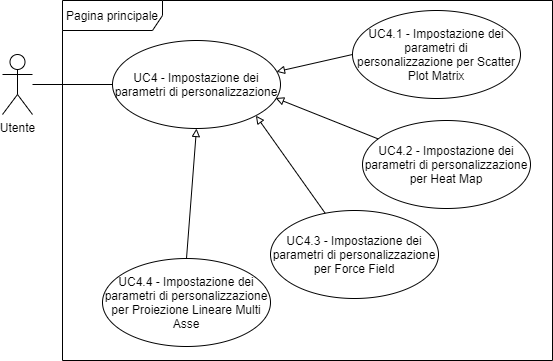
\includegraphics[width=9cm]{Section/Images/UC4.png}
\centering
\caption{UC4 - Modifica della riduzione dimensionale tramite algoritmo}
\end{figure}
\begin{itemize}
	\item \textbf{Attore primario}: Utente;
	\item \textbf{Precondizioni}: L'utente ha scelto l'algoritmo di riduzione dimensionale [UC3.1];
	\item \textbf{Postcondizioni}: I parametri di personalizzazione dell'algoritmo sono stasi impostati e vengono create il numero di dimensioni scelte, pronte per essere visualizzare [UC5];
	\item \textbf{Scenario principale}: L'utente
	
	\begin{enumerate}
		\item Seleziona il numero di dimensioni da ricavare dalla riduzione dimensionale [UC4.1];
		\item Personalizza i parametri dell'algoritmo di riduzione dimensionale selezionato secondo le sue esigenze [UC4.2].
	\end{enumerate}		
\end{itemize}

\subsubsection{UC4.1 - Selezione del numero di dimensioni}

\begin{itemize}
	\item \textbf{Attore primario}: Utente;
	
	\item \textbf{Precondizioni}: L'utente ha scelto un algoritmo di riduzione dimensionale [UC3.1];
	
	\item \textbf{Postcondizioni}: L'utente ha selezionato il numero di dimensioni che vuole ottenere dal processo di riduzione dimensionale;
	
	\item \textbf{Scenario principale}: L'utente decide il numero di dimensioni da ricavare selezionando un numero tra l'intervallo disponibile.
\end{itemize}	
	
\newpage	
	
\subsubsection{UC4.2 - Impostazione dei parametri dell'algoritmo}
\begin{figure}[h]
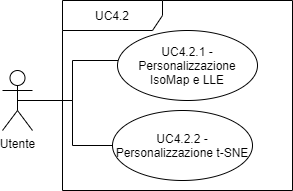
\includegraphics[width=9cm]{Section/Images/UC4.2.png}
\centering
\caption{UC4.2 - Impostazione dei parametri dell'algoritmo}
\end{figure}
\begin{itemize}
	\item \textbf{Attore primario}: Utente;
	
	\item \textbf{Precondizioni}: L'utente ha scelto un algoritmo di riduzione dimensionale [UC3.1];
	
	\item \textbf{Postcondizioni}: L'utente ha impostato i parametri personalizzabili dell'algoritmo;
	
	\item \textbf{Scenario principale}: L'utente imposta i parametri specifici dell'algoritmo selezionato.
	
		\item \textbf{Generalizzazioni}: L'utente imposta i parametri di personalizzazione dell'algoritmo scelto:
	\begin{enumerate}[(a)]
		\item Personalizzazione \glo{\textit{IsoMap}} e \glo{\textit{LLE}} [UC4.2.1];
		\item Personalizzazione \glo{\textit{t-SNE}} [UC4.2.2];
	\end{enumerate}
\end{itemize}		
		

\subsubsection{UC4.2.1 - Personalizzazione IsoMap e LLE}
\begin{itemize}
	\item \textbf{Attore primario}: Utente;
	
	\item \textbf{Precondizioni}: L'utente ha scelto l'algoritmo \textit{IsoMap} [UC3.1.1] oppure \textit{LLE} [UC3.1.2];
	
	\item \textbf{Postcondizioni}: L'algoritmo viene impostato con le personalizzazioni dell'utente;
	
	\item \textbf{Scenario principale}: L'utente seleziona il numero di punti vicini (\glo{\textit{neighbors}}), tra l'intervallo disponibile, per la stima approssimativa del \glo{\textit{manifold}}.

\end{itemize}

\newpage

\subsubsection{UC4.2.2 - Personalizzazione t-SNE}
\begin{figure}[h]
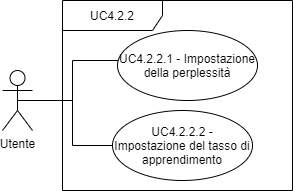
\includegraphics[width=9cm]{Section/Images/UC4.2.2.png}
\centering
\caption{UC4.2.2 - Personalizzazione t-SNE}
\end{figure}
\begin{itemize}
	\item \textbf{Attore primario}: Utente;
	
	\item \textbf{Precondizioni}: L'utente ha scelto l'algoritmo \textit{t-SNE} [UC3.1.4];
	
	\item \textbf{Postcondizioni}: L'algoritmo viene impostato con le personalizzazioni dell'utente;
	
	\item \textbf{Scenario principale}: L'utente decide:

\begin{enumerate}
\item Impostazione della perplessità [UC4.2.2.1];
\item Impostazione del tasso di apprendimento (\glo{\textit{Epsilon}}) [UC4.2.2.2];
\end{enumerate}	

\end{itemize}
	
	
\paragraph{UC4.2.2.1 - Impostazione della perplessità}
\begin{itemize}
	\item \textbf{Attore primario}: Utente;
	
	\item \textbf{Precondizioni}: L'utente ha scelto l'algoritmo \textit{t-SNE} [UC3.1.4];
	
	\item \textbf{Postcondizioni}: L'algoritmo viene impostato con le personalizzazioni dell'utente;
	
	\item \textbf{Scenario principale}: L'utente imposta il valore, tra l'intervallo disponibile, per bilanciare gli aspetti globali e locali dei dati.

\end{itemize}
	
\paragraph{UC4.2.2.2 - Impostazione del tasso di apprendimento}
\begin{itemize}
	\item \textbf{Attore primario}: Utente;
	
	\item \textbf{Precondizioni}: L'utente ha scelto l'algoritmo \textit{t-SNE} [UC3.1.4];
	
	\item \textbf{Postcondizioni}: L'algoritmo viene impostato con le personalizzazioni dell'utente;
	
	\item \textbf{Scenario principale}: L'utente imposta il valore, tra l'intervallo disponibile, del tasso di apprendimento dell'algoritmo.

\end{itemize}

\subsubsection{UC4.3 - Assegnazione del nome alle dimensioni create}

\begin{itemize}
	\item \textbf{Attore primario}: Utente;
	
	\item \textbf{Precondizioni}: L'utente ha scelto un algoritmo di riduzione dimensionale [UC3.1];
	
	\item \textbf{Postcondizioni}: L'utente ha assegnato i nomi alle dimensioni che andrà a creare;
	
	\item \textbf{Scenario principale}: L'utente assegna il nome alle dimensioni che sta creando nell'apposito campo d'input; il nome scelto sarà seguito da un numero crescente, che dipende dal numero di dimensioni generate. Se non modificato vengono mantenuti i nomi di default, costituiti dal nome dell'algoritmo scelto.

\end{itemize}	

\subsubsection{UC4.1 Personalizzazione Scatter Plot Matrix}
\begin{itemize}
	\item \textbf{Attore primario}: Utente.
	\item \textbf{Precondizioni}: L'utente ha selezionato la visualizzazione \textit{Scatter Plot Matrix} [UC3.1] e il sistema la rappresenta.
	\item \textbf{Postcondizioni}: L'utente visualizza il grafico con le modifiche apportate.
	\item \textbf{Scenario principale}:
	\begin{enumerate}
			\item Viene presentata all'utente una sezione per apportare delle modifiche allo \textit{Scatter Plot Matrix} appena visualizzato;
			\item L'utente decide le dimensioni da visualizzare e dove posizionarle nel grafico;
			\item Al termine, l'utente dovrà premere sul pulsante per la conferma e l'invio delle nuove preferenze.
		\end{enumerate}
\end{itemize}
\subsubsection{UC4.2 Impostazione dei parametri di personalizzazione per Heat Map}
\begin{itemize}
	\item \textbf{Attore primario}: Utente.
	\item \textbf{Precondizioni}: L'utente ha selezionato la visualizzazione \textit{Heat Map} [UC3.2] e il sistema la rappresenta.
	\item \textbf{Postcondizioni}: Viene aggiornata la visualizzazione \textit{Heat Map} con i nuovi parametri impostati dall'utente.
	\item \textbf{Scenario principale}:
	\begin{enumerate}
			\item Viene presentata all'utente una sezione per apportare delle modifiche ai parametri relativi alla visualizzazione \textit{Heat Map};
			\item L'utente decide le dimensioni da utilizzare e il tipo di distanza da calcolare;
			\item Al termine, l'utente dovrà premere sul pulsante per la conferma e l'invio delle nuove preferenze.
		\end{enumerate}
\end{itemize}
\subsubsection{UC4.3 - Impostazione dei parametri di personalizzazione per Force Field}
\begin{itemize}
	\item \textbf{Attore primario}: Utente.
	\item \textbf{Precondizioni}: L'utente ha selezionato la visualizzazione \glo{\textit{Force Field}} [UC3.3] e il sistema la rappresenta.
	\item \textbf{Postcondizioni}: Viene aggiornata la visualizzazione \glo{\textit{Force Field}} con i nuovi parametri impostati dall'utente.
	\item \textbf{Scenario principale}:
	\begin{enumerate}
			\item Viene presentata all'utente una sezione per apportare delle modifiche ai parametri relativi alla visualizzazione \glo{\textit{Force Field}};
			\item L'utente decide le dimensioni da utilizzare e il tipo di distanza da calcolare;
			\item Al termine, l'utente dovrà premere sul pulsante per la conferma e l'invio delle nuove preferenze.
		\end{enumerate}
\end{itemize}
\subsubsection{UC4.4 Personalizzazione Proiezione Lineare Multi Asse}
\begin{itemize}
	\item \textbf{Attore primario}: Utente.
	\item \textbf{Precondizioni}: L'utente ha selezionato la visualizzazione \textit{Proiezione Lineare Multi Asse} [UC3.4] e il sistema la rappresenta.
	\item \textbf{Postcondizioni}: L'utente visualizza il grafico con le modifiche apportate.
	\item \textbf{Scenario principale}:
	\begin{enumerate}
			\item Viene presentata all'utente una sezione per apportare delle modifiche al grafico di tipo \textit{Proiezione Lineare Multi Asse} appena visualizzato;
			\item L'utente decide le dimensioni da visualizzare;
			\item Al termine, l'utente dovrà premere sul pulsante per la conferma e l'invio delle nuove preferenze.
		\end{enumerate}
\end{itemize}
\subsection{UC5 - Scelta della \glo{visualizzazione}}
\begin{figure}[h]
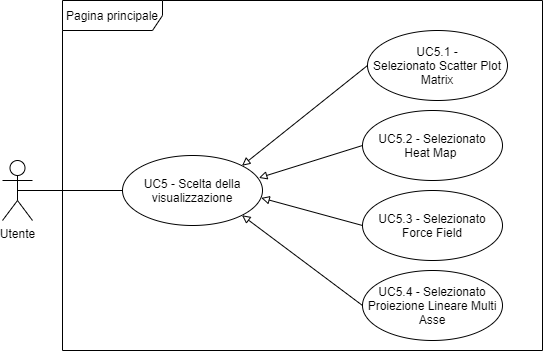
\includegraphics[width=\linewidth]{Section/Images/UC5.png}
\centering
\caption{UC5 - Scelta della visualizzazione}
\end{figure}
\begin{itemize}
	\item \textbf{Attore primario}: Utente;
	\item \textbf{Precondizioni}: L'utente ha caricato dei dati nel sistema e ha selezionato le dimensioni da utilizzare [UC2].
	\item \textbf{Postcondizioni}: Viene mostrata la visualizzazione scelta, con possibilità di personalizzazione [UC6]. La scelta viene salvata nel sistema.
	\item \textbf{Scenario principale}: L'utente seleziona la visualizzazione che vuole utilizzare tra quelle disponibili.
	\item \textbf{Generalizzazioni}: L'utente seleziona una delle seguenti opzioni:
		\begin{enumerate}
			\item \glo{\textit{Scatter Plot Matrix}} [UC5.1];
			\item \glo{\textit{Heat Map}} [UC5.2];
			\item \glo{\textit{Force Field}} [UC5.3];
			\item \glo{\textit{Proiezione Lineare Multi Asse}} [UC5.4].
		\end{enumerate}

\end{itemize}
\newpage
\subsection{UC6 - Personalizzazione della visualizzazione}
\begin{figure}[h]
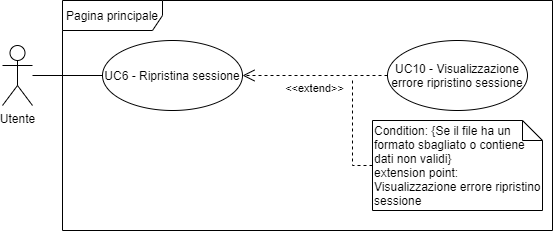
\includegraphics[width=\linewidth]{Section/Images/UC6.png}
\centering
\caption{Diagramma sulla personalizzazione della visualizzazione scelta}
\end{figure}
\begin{itemize}
	\item \textbf{Attore primario}: Utente;
	
	\item \textbf{Precondizioni}: L'utente ha scelto il grafico tra quelli a disposizione nel sistema [UC5];
	
	\item \textbf{Postcondizioni}: Il grafico viene aggiornato con le personalizzazioni impostate dall'utente;
	
	\item \textbf{Scenario principale}: L’utente sceglie come impostare le opzioni di personalizzazione del grafico. Verranno applicati, per ciascun campo, dei valori di default che l'utente può decidere di modificare o meno. In caso fosse stato precedentemente caricato un file di ripristino sessione [UC1.2] i valori di default iniziali diventerebbero quindi quelli specificati in questo file, lasciando comunque all'utente la possibilità di modificarli;
	
	\item \textbf{Generalizzazioni}: L'utente imposta i parametri di personalizzazione della visualizzazione scelta:
	\begin{enumerate}[(a)]
	\item Personalizzazione \textit{Scatter Plot Matrix} [UC6.1];
	\item Personalizzazione \textit{Adjacency Matrix} [UC6.2];
	\item Personalizzazione \textit{Force Field} [UC6.3];
	\item Personalizzazione \textit{Proiezione Lineare Multi Asse} [UC6.4];
	\item Personalizzazione \textit{Heat Map} [UC6.5].
	\end{enumerate}
		
\end{itemize}



\subsubsection{UC7 - Salva sessione}
\begin{itemize}
	\item \textbf{Attore primario}: Utente.
	\item \textbf{Precondizioni}: L'utente ha caricato dei dati nel sistema [UC1] e ha scelto il tipo di grafico da visualizzare [UC5]
	\item \textbf{Postcondizioni}: L'utente possiede un file \glo{JSON} per il ripristino della sessione.
	\item \textbf{Scenario principale}:
		\begin{enumerate}
			\item L'utente ha una sessione di lavoro aperta.
			\item L'utente seleziona la funzionalità "salva sessione";
			\item L'utente seleziona la directory in cui salvare il file.
		\end{enumerate}
\end{itemize}
\subsection{UC8 - Personalizzazione Force Field}
\begin{itemize}
	\item \textbf{Attore primario}: Utente.
	
	\item \textbf{Precondizioni}: L'utente ha scelto il grafico \textit{Force Field} [UC5.3].
	
	\item \textbf{Postcondizioni}: Il grafico viene aggiornato.
	
	\item \textbf{Scenario principale}: L'utente visualizza:
	
\begin{enumerate}
	\item Una lista con le funzioni di forza fornite dal sistema e può scegliere quale utilizzare tra quelle disponibili; 
	\item Una lista con tutte i tipi di distanza disponibili nel sistema e può scegliere quale utilizzare per il calcolo. 
\end{enumerate}	
	Inoltre l'utente può decidere alcuni stili del grafico, tra cui:
		\begin{enumerate}
			\item Scegliere quale dimensione utilizzare per il colore dei punti nel grafico;
				
			\item Scegliere quale dimensione utilizzare per la forma dei punti nel grafico;
			
			\item Scegliere quale dimensione utilizzare per l'etichetta dei punti nel grafico;
			
			\item Scegliere quale dimensione utilizzare per la dimensione dei punti nel grafico;
				
		\end{enumerate}
		
	\item \textbf{Estensioni}:
	\begin{enumerate}[(a)]
		\item ...
	\end{enumerate}
\end{itemize}


\subsubsection{UC9 - Personalizzazione Proiezione Lineare Multi Asse}
\begin{itemize}
	\item \textbf{Attore primario}: Utente.
	
	\item \textbf{Precondizioni}: L'utente ha scelto il grafico \textit{Proiezione Lineare Multi Asse} [UC5.4].
	
	\item \textbf{Postcondizioni}: Il grafico viene aggiornato.
	
	\item \textbf{Scenario principale}: L'utente sceglie che dimensioni visualizzare nel grafico tra quelle a disposizione. Inoltre può decidere alcune stili del grafico, tra cui:
		\begin{enumerate}
			\item Scegliere quale dimensione utilizzare per il colore dei punti nel grafico;
				
			\item Scegliere quale dimensione utilizzare per la forma dei punti nel grafico;
			
			\item Scegliere quale dimensione utilizzare per l'etichetta dei punti nel grafico;
			
			\item Scegliere quale dimensione utilizzare per la dimensione dei punti nel grafico;
				
		\end{enumerate}
		
	\item \textbf{Estensioni}:
	\begin{enumerate}[(a)]
		\item ...
	\end{enumerate}
\end{itemize}
\subsection{UC10 - Visualizzazione errore scelta dimensioni}
\begin{itemize}
	\item \textbf{Attore primario}: Utente;
	\item \textbf{Precondizioni}: L'utente non ha selezionato alcuna dimensione tra quelle presenti nel dataset precedentemente caricato;
	\item \textbf{Postcondizioni}: L'utente visualizza un messaggio di errore esplicativo;
	\item \textbf{Scenario principale}:
		\begin{enumerate}
			\item L'utente visualizza un messaggio di errore esplicativo;
			\item L'utente clicca "OK" per continuare.
		\end{enumerate}
\end{itemize}
\newpage
\section{Requisiti minimi di sistema}
Per poter utilizzare l'applicazione web HDViz è necessario avere i seguenti requisiti:
\subsection{Prerequisiti}
\begin{itemize}
	\item Node.js v14.16.0 LTS o v15.12.0;
	\item Npm v6.x o v7.x;
\end{itemize}
\subsection{Requisiti hardware}
\begin{itemize}
	
	\item Processore (CPU): Dual core a 2Ghz;
	\item Memoria (RAM): 4GB;
	\item Connessione internet: attiva (7 Mb/s);
\end{itemize}

\subsection{Requisiti software}
\begin{itemize}
	\item Sistema operativo: Windows 10, Debian, Ubuntu, MacOs;
	\begin{itemize}
		\item  \textit{Windows} 10;
		\item \textit{Debian} dalla versione 9 in poi;
		\item \textit{Ubuntu} versione 20.04 LTS o 20.10
		\item \textit{MacOs} dalla versione 10.13 High Sierra in poi.
	\end{itemize}
	\item Browser: 
	\begin{itemize}
		\item  \textit{Google Chrome} dalla versione 75.0 in poi;
		\item \textit{Mozilla Firefox} dalla versione 69.0 in poi;
		\item \textit{Microsoft Edge} dalla versione 81.0.416 in poi;
		\item \textit{Safari} dalla versione 13.1 in poi.
	\end{itemize}	 
\end{itemize}

\end{document}